\section{Athermal phonons in the substrate}\label{sec:20.2}

At the partition time of \cref{sec:19.1}, some \SI{100}{ps} after a \SI{100}{eV} electron recoil in silicon, about \SI{69}{eV} sits in phonons of tens of meV, some two thousand of them near the point of the event. A sensor film on the surface absorbs phonons microseconds later, after they have decayed several times and scattered off isotopes hundreds of times. The phonons of a nuclear recoil of the same energy start from a different spectrum. If that difference survived to the sensor, a phonon readout could tell the two recoils apart by what it absorbs, and the phonon collection of a nuclear recoil could differ from that of the electron recoil used to calibrate it (\cref{sec:19.5}). Two rates decide the question: anharmonic decay, which scales as the fifth power of the phonon energy, and isotope scattering, which scales as the fourth. Together they drive every hard spectrum toward one shape that depends on time only through a single energy scale, and they leave the energy born at low phonon energies as the difference that a linear readout can still see.

\subsection{Prompt phonons at the partition time}\label{sec:20.2-prompt}

The phonons that carry the prompt energy $E_{\mathrm{prompt}} = E_{\mathrm{phon}}(t_{\mathrm{pr}})$ of \cref{sec:19.5-law} are \emph{athermal}. Their energies $E_{\mathrm{ath}}$, from meV to tens of meV, exceed the thermal energy of \SI{0.86}{\micro eV} at \SI{10}{mK} by four orders of magnitude or more, and their population is far from equilibrium. It is also dilute: about 2300 phonons of \SI{30}{meV}, even if confined to a sphere of radius \SI{1}{\micro m}, share $6\times10^{11}$ modes, an occupation of $4\times10^{-9}$. They do not interact with each other. Each phonon interacts with the static crystal alone, scattering off the random isotope masses, and decays spontaneously through the cubic anharmonicity; at \SI{10}{mK} the Bose factors of \cref{eq:5.7-gamma} vanish, leaving spontaneous decay. The transport is linear in the deposit, and the birth spectrum is the initial condition of a linear evolution.

The two recoils make their phonons in different ways. In an electron recoil the hot carriers of \cref{chap:18} lose most of their energy by emitting optical and intervalley phonons (\cref{sec:18.1-ph}). An optical phonon lives \SI{3.7}{ps} (\cref{we:5-klemens}) and decays mostly into a longitudinal acoustic phonon near \SI{42}{meV} and a transverse one near \SI{22}{meV} (\cref{sec:5.7}). By $t_{\mathrm{pr}}$ the optical phonons are gone, and the population is acoustic and hard. Below the optical energy a carrier can emit only acoustic phonons, and momentum conservation caps their energy at $2c_{\mathrm{LA}}k$ for a carrier of momentum $k$. For a silicon electron with the density-of-states mass $0.32\,m_e$ of one valley, the cap is \SI{8.7}{meV} at a kinetic energy of \SI{64}{meV} and \SI{6.0}{meV} at \SI{30}{meV}. Suppose each carrier enters this regime with a kinetic energy spread uniformly below $\omega_{\mathrm{opt}}$. Each of the two carriers then has the mean kinetic energy $\omega_{\mathrm{opt}}/2$, so each pair sheds on average $\omega_{\mathrm{opt}}$ in phonons below about 6 to \SI{9}{meV}, and the soft fraction of the deposit is
\begin{equation}
  f_{\mathrm{s}} \simeq \frac{\omega_{\mathrm{opt}}}{\varepsilon_{\mathrm{eh}}} .
  \label{eq:20.2-fs}
\end{equation}
This estimate gives \SI{1.7}{\percent} in silicon, with the measured $\omega_{\mathrm{opt}} = \SI{64.1}{meV}$ (\cref{sec:5.2}) and $\varepsilon_{\mathrm{eh}} = \SI{3.75}{eV}$ (\cref{sec:18.2}), and \SI{1.3}{\percent} in germanium, with \SI{37.6}{meV} (\cref{tab:5-phonons}) and \SI{2.96}{eV}~\cite[Table~I]{leman2012invited}. The gap energy $N_{\mathrm{eh}}\Eg$, \SI{31}{\percent} of an electron recoil in silicon, is not part of the prompt population. It returns as phonons later, where and with which spectrum the release channel decides (\cref{sec:19.5,sec:20.5}).

In a nuclear recoil below the displacement threshold the whole deposit is heat (\cref{sec:19.1}). For small recoils the phonons that the nuclear response creates are the final state, with the energy-weighted phonon content of \cref{sec:11.3}. Above a few eV the created spectrum comes from the molecular dynamics of \cref{app:E.23}, which has not been tabulated. A recoil that thermalizes locally fills the modes in proportion to their density of states, and its spectrum is hard as well. Both populations are hard, between about 4 and \SI{15}{THz} in silicon, and they differ in branch content and in shape; only the electron recoil carries the soft fraction $f_{\mathrm{s}}$.

\subsection{Anharmonic down-conversion}\label{sec:20.2-anh}

The linewidth \cref{eq:5.7-gamma} at $T = 0$ gives the decay rate of any phonon. For an acoustic phonon of long wavelength it takes a simple form, because both of its ingredients, the vertex and the phase space, scale as powers of the frequency. Translation invariance makes the vertex small. By the sum rule \cref{eq:5.7-asr}, the third-order constants vanish when summed over the positions of any one atom. In \cref{eq:5.7-V3} the term of zeroth order in each wavevector cancels whenever the polarizations are those of a uniform translation, as they are for acoustic phonons at small $Q$. The first surviving term carries one power of each wavevector, $Q_1Q_2Q_3$, multiplied by the third-order elastic constants. With the prefactor $(\omega_1\omega_2\omega_3)^{-1/2}$ and the linear dispersion $\omega_i = c_iQ_i$, the vertex becomes
\begin{equation}
  V^{(3)}(1,2,3) = (\omega_1\omega_2\omega_3)^{1/2}\,v_3(\hat{\vect{Q}}_i, \nu_i) ,
  \label{eq:20.2-V3}
\end{equation}
with $v_3$ a function of the directions and branches alone. The squared vertex of a decay $\omega \to \omega_1 + \omega_2$ is then $\omega^3y(1 - y)|v_3|^2$, with $y = \omega_1/\omega$. The phase space is the sum over $\vect{Q}_1$ at fixed $\vect{Q}_2 = \vect{Q} - \vect{Q}_1$. In polar coordinates about $\vect{Q}$, the angle integral of the energy delta function is $\int\dd\cos\theta\,\delta(\omega - c_1Q_1 - c_2Q_2) = Q_2/(c_2QQ_1)$, since $\dd Q_2/\dd\cos\theta = -QQ_1/Q_2$. The remaining integral $(2\pi/c_2Q)\int\dd Q_1\,Q_1Q_2$ scales as $\omega^2$. The angles at which the decay happens are fixed by $y$ and the speeds, so $v_3$ contributes a function of $y$ only, and the rate scales as $\omega^3\times\omega^2$:
\begin{equation}
  \varGamma_{\mathrm{anh}} = A_{\mathrm{anh}}\Bigl(\frac{E_{\mathrm{ath}}}{h}\Bigr)^5 .
  \label{eq:20.2-anh}
\end{equation}
This is \cref{eq:E.12-anh}. The constant $A_{\mathrm{anh}}$ depends on the second- and third-order elastic constants and on the branch of the decaying phonon. The derivation needs normal processes ($\vect{G} = 0$) and frequencies low enough for linear dispersion, the same long-wavelength condition as for the Rayleigh law of isotope scattering below.

Not every branch decays. In the isotropic continuum a transverse phonon cannot decay at all. Its energy $c_{\mathrm{T}}Q$ would have to equal $c_1Q_1 + c_2Q_2$, with both speeds at least $c_{\mathrm{T}}$, the lowest speed, and with $Q_1 + Q_2 \ge Q$ by the triangle inequality. The only solutions are collinear decays into two transverse phonons, for which the isotropic vertex vanishes. A longitudinal phonon decays through the channels $\mathrm{L}\to\mathrm{L}'+\mathrm{T}'$ and $\mathrm{L}\to\mathrm{T}+\mathrm{T}$, with the daughter energies distributed as in \cref{app:E.12}. Anisotropy and dispersion open slow decays of transverse phonons in real crystals, which transport codes neglect~\cite[Sect.~2.2.2]{kelsey2023g4cmp}. In the isotropic continuum $A_{\mathrm{anh}}$ is a closed form in five elastic constants, the two Lamé constants and three third-order combinations~\cite[Eqs.~(1), (2)]{hernandez2025modeling}. For silicon, Tamura's calculation gives $A_{\mathrm{anh}} = \SI{7.41e-56}{s^4}$~\cite[Table~I]{leman2012invited}, and a recalculation from cryogenic elastic constants gives \SI{1.15e-55}{s^4}~\cite[Table~3]{hernandez2025modeling}. For germanium the published values spread over a factor of ten, from \SI{1.61e-55}{s^4}~\cite{hertel2012phonon} through \SI{6.8e-55}{s^4} in the recalculation to \SI{1.65e-54}{s^4}. Two of them are both attributed to Tamura's work yet disagree by a factor 2.6: \SI{6.43e-55}{s^4}~\cite[Table~I]{leman2012invited} and \SI{1.65e-54}{s^4}~\cite[Table~3]{hernandez2025modeling}. No direct measurement exists for either crystal, and we use the slowest germanium value, \SI{1.61e-55}{s^4}. A longitudinal phonon at the top of the silicon acoustic band, \SI{15}{THz}, decays in \SI{18}{ps}; one at \SI{1}{THz} lives \SI{14}{\micro s}.

The constants come from the elastic tensors. The second-order constants are measured or computed as in \cref{app:E.4}; the third-order ones follow from the same finite-strain calculations taken one order further, or from ultrasonic measurements under stress. \Cref{app:E.12} sets out how the two rates enter a transport Monte Carlo of a whole detector, together with the kinematics of the daughters and the focusing of the group velocities. \Cref{app:E.25} specifies how the created-phonon spectra of the two recoils are carried through it to the sensors.

\subsection{Isotope scattering}\label{sec:20.2-iso}

Natural silicon is \SI{92.2}{\percent} $^{28}$Si, \SI{4.7}{\percent} $^{29}$Si and \SI{3.1}{\percent} $^{30}$Si, and a phonon sees the random masses as point scatterers. Write the isotope on site $I$ as a mass defect $\delta^M_I = (\bar M - M_I)/\bar M$ about the mean mass $\bar M$, whose variance over the isotopes is the mass variance $g_{\mathrm{md}} = \sum_ix_i(\delta^M_i)^2$ of \cref{app:E.12}. To lowest order in $g_{\mathrm{md}}$, the self-energy of the mass disorder in \cref{sec:11.6} gives every phonon of frequency $\omega$ the same width,
\begin{equation}
  \varGamma_{\mathrm{iso}}(\omega) = \frac{\pi}{6}\,g_{\mathrm{md}}\,\omega^2\,g_{\mathrm{ph},\kappa}(\omega) ,
  \label{eq:20.2-isoborn}
\end{equation}
with $g_{\mathrm{ph},\kappa}$ the site-projected density of states normalized to three. The polarization of the initial phonon drops out because on a site of cubic symmetry, as in silicon, the polarization sum over final states is isotropic: cubic symmetry makes the tensor $N^{-1}\sum_{\vect{Q}'\nu'}e^{\beta}_{\kappa\nu'}e^{\gamma*}_{\kappa\nu'}\delta(\omega - \omega_{\vect{Q}'\nu'})$ proportional to $\delta_{\beta\gamma}$, and the normalization fixes the factor $g_{\mathrm{ph},\kappa}/3$. At low frequency the density of states takes its Debye form, $g_{\mathrm{ph},\kappa} = 3\Omega_{\mathrm{at}}\omega^2\langle c^{-3}\rangle/2\pi^2$, with $\Omega_{\mathrm{at}}$ the volume per atom and $\langle c^{-3}\rangle$ the average of $\frac13\sum_\nu c_\nu^{-3}$ over directions. \Cref{eq:20.2-isoborn} then becomes the Rayleigh law
\begin{equation}
  \varGamma_{\mathrm{iso}} = B_{\mathrm{iso}}\Bigl(\frac{E_{\mathrm{ath}}}{h}\Bigr)^4 , \qquad
  B_{\mathrm{iso}} = 4\pi^3g_{\mathrm{md}}\,\Omega_{\mathrm{at}}\langle c^{-3}\rangle ,
  \label{eq:20.2-rayleigh}
\end{equation}
which is \cref{eq:E.12-iso} and Tamura's result~\cite[Eq.~(4)]{hernandez2025modeling}. Isotope scattering conserves energy. In the isotropic continuum it also forgets the branch, since the final branch is drawn with a weight proportional to its density of states whatever the initial one. Repeated scattering holds the branches at their equilibrium shares, with a longitudinal share $f_{\mathrm{LA}}$ of \SI{9.3}{\percent} in silicon and \SI{9.8}{\percent} in germanium~\cite[Sect.~2.2.2]{kelsey2023g4cmp}, set by the density of states of the anisotropic crystal (the isotropic speeds of \cref{app:C.18} would give \SI{9.75}{\percent} in silicon).

\begin{workedexample}{The isotope rate of natural silicon at \SI{1}{THz}}\label{we:20-iso}
With the AME2020 masses and the natural abundances, $\bar M = \SI{28.0855}{u}$, and the three isotopes have the mass defects $\delta^M = +0.39$, $-3.17$ and $\SI{-6.72}{\percent}$~\cite{wang2021ame2020,meija2016isotopic}. Their contributions to $g_{\mathrm{md}}$ are $1.38\times10^{-5}$, $4.72\times10^{-5}$ and $1.40\times10^{-4}$, so $g_{\mathrm{md}} = 2.007\times10^{-4}$, and $^{30}$Si, the rarest isotope, carries \SI{70}{\percent} of it. The volume per atom is $a^3/8 = \SI{20.02}{\angstrom^3}$. Averaging $\frac13\sum_\nu c_\nu^{-3}$ over directions with the measured elastic tensor of \cref{app:C.18} gives $\langle c^{-3}\rangle = \SI{4.90e-12}{s^3.m^{-3}}$. The isotropic code speeds of \cref{app:E.12}, 9.0 and \SI{5.4}{km/s}, give \SI{4.69e-12}{s^3.m^{-3}}, \SI{4}{\percent} less, because they miss the slow transverse wave along $[110]$. Then
\begin{equation*}
  B_{\mathrm{iso}} = 124.0\times(2.007\times10^{-4})\times(\SI{2.002e-29}{m^3})\times(\SI{4.90e-12}{s^3.m^{-3}}) = \SI{2.44e-42}{s^3} .
\end{equation*}
This lies inside the range 2.42 to \SI{2.56e-42}{s^3} that Tamura, Shields, Ramsbey and Wolfe measured across the phonon polarizations~\cite[Table~4]{hernandez2025modeling}. At $E_{\mathrm{ath}}/h = \SI{1}{THz}$, or \SI{4.14}{meV}, the rate is $\varGamma_{\mathrm{iso}} = \SI{2.44e6}{s^{-1}}$: a lifetime of \SI{0.41}{\micro s}, and $3.9\times10^{-7}$ of the angular frequency. With the rms group speed of the mixed branches, \SI{5.85}{km/s} for the code speeds, the mean free path is \SI{2.4}{mm}, comparable with the thickness of a detector and some $4\times10^5$ transverse wavelengths. The full density of states raises the rate at \SI{1}{THz} by about \SI{5}{\percent} above the Rayleigh law (\cref{lim:20.2b}). Germanium has $g_{\mathrm{md}} = 5.87\times10^{-4}$ from the same tables and slower sound, and $B_{\mathrm{iso}} = \SI{3.67e-41}{s^3}$~\cite[Table~I]{leman2012invited}, fifteen times that of silicon.
\end{workedexample}

The Rayleigh law fails early in silicon. \Cref{lim:20.2b} compares it with \cref{eq:20.2-isoborn} evaluated with the density of states of the PBE force constants of \cref{sec:5.2}, integrated over the zone on rays from $\mathrm{\Gamma}$ so that small $Q$ is sampled finely. The ratio of the two rates is $g_{\mathrm{ph},\kappa}/g_{\mathrm{Debye}}$, independent of $g_{\mathrm{md}}$. For the comparison the Debye density uses the PBE sound speeds, whose $\langle c^{-3}\rangle$ is \SI{22}{\percent} above the measured one because PBE makes the transverse branches soft; the absolute rate is that of \cref{we:20-iso}. The transverse branches bend over well before the zone boundary. The density of states, and with it the rate, exceeds the Rayleigh law by \SI{10}{\percent} already at \SI{5.6}{meV}, or \SI{1.36}{THz}, a tenth of the Debye energy $\omega_{\mathrm{D}} = \SI{55.6}{meV}$.

\begin{limitbox}[Rayleigh law of isotope scattering][lim:20.2b]
The published rate is $\varGamma_{\mathrm{iso}} = B_{\mathrm{iso}}(E_{\mathrm{ath}}/h)^4$ with $B_{\mathrm{iso}} = 4\pi^3g_{\mathrm{md}}\Omega_{\mathrm{at}}/\langle c^{3}\rangle$, $\langle c^{3}\rangle$ the polarization-averaged cubed sound speed~\cite[Eq.~(4)]{hernandez2025modeling}. The book uses the average of the inverse cube, $\langle c^{-3}\rangle$, which is what the Debye density of states contains; the two forms agree when the three speeds are equal.
\par\smallskip
{\centering
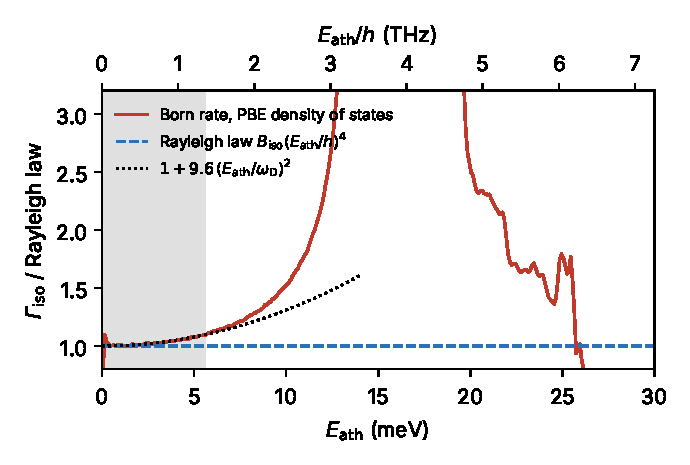
\includegraphics[width=0.75\linewidth]{figures/ch20/limit20_2b.pdf}
\captionof{figure}{Isotope scattering rate of silicon from the Born rate \cref{eq:20.2-isoborn} with the full density of states (red), divided by the Rayleigh law \cref{eq:20.2-rayleigh} (dashed, one), against the phonon energy (lower axis) and frequency (upper axis). The ratio is $g_{\mathrm{ph},\kappa}(\omega)/g_{\mathrm{Debye}}(\omega)$, independent of the mass variance. Density of states from the PBE force constants of \cref{sec:5.2}, integrated in spherical coordinates about $\mathrm{\Gamma}$ to the zone boundary (32 Gauss--Legendre polar points, 64 azimuths, 800 radial steps, \SI{0.1}{meV} bins, running mean over three bins); the Debye reference uses the PBE sound speeds. Dotted: the leading correction $1 + 9.6\,(E_{\mathrm{ath}}/\omega_{\mathrm{D}})^2$, fitted between 2 and \SI{6}{meV}, with $\omega_{\mathrm{D}} = \SI{55.6}{meV}$. Gray: within \SI{10}{\percent} of the Rayleigh law, $E_{\mathrm{ath}} \le \SI{5.6}{meV}$. The ratio peaks at 8.1 near \SI{17.6}{meV}, above the plotted range.}\label{fig:20-limit-iso}
\par}
\smallskip
Above \SI{1.4}{THz} the transverse branches of silicon are no longer linear, and the rate follows the density of states rather than the fourth power of the frequency.
\end{limitbox}

\subsection{The scaling spectrum}\label{sec:20.2-scaling}

The two rates set up a hierarchy. For a longitudinal phonon their ratio is $B_{\mathrm{iso}}/A_{\mathrm{anh}}$ divided by the frequency, and $B_{\mathrm{iso}}/A_{\mathrm{anh}}$ is \SI{33}{THz} in silicon and \SI{228}{THz} in germanium with its slowest decay. A phonon scatters off isotopes more often than it decays, by a factor 3.3 at \SI{10}{THz} in silicon and by more at lower frequency. Between two decays the branches stay close to their equilibrium shares, and a phonon of any branch spends the fraction $f_{\mathrm{LA}}$ of its time as a longitudinal phonon, the only branch that decays. The population decays at the mean rate $f_{\mathrm{LA}}\varGamma_{\mathrm{anh}}$, and isotope scattering, which conserves energy, drops out of the evolution of the energy spectrum. Let $\rho_E(E_{\mathrm{ath}}, t)$ be the energy per unit phonon energy, and $P_{\mathrm{d}}(y)$ the energy-weighted distribution of the fraction $y$ that a decay passes to a daughter, counting both daughters: with $p(y)$ the number density of one daughter, $P_{\mathrm{d}}(y) = 2y\,p(y)$, so that $\int_0^1P_{\mathrm{d}}(y)\,\dd y = 1$. Energy flows only downward:
\begin{equation}
  \frac{\partial\rho_E(E,t)}{\partial t} = -f_{\mathrm{LA}}\varGamma_{\mathrm{anh}}(E)\,\rho_E(E,t)
  + \int_E^\infty\frac{\dd E'}{E'}\,P_{\mathrm{d}}\Bigl(\frac{E}{E'}\Bigr)\,f_{\mathrm{LA}}\varGamma_{\mathrm{anh}}(E')\,\rho_E(E',t) .
  \label{eq:20.2-frag}
\end{equation}
In the isotropic continuum $P_{\mathrm{d}}$ depends on the energy ratio alone, as the distribution of \cref{app:E.12} does, since the kinematics of a decay contain no energy scale. The rate \cref{eq:20.2-anh} contains one scale, which combines with the time into
\begin{equation}
  E_*(t) = h\,(f_{\mathrm{LA}}A_{\mathrm{anh}}t)^{-1/5} , \qquad
  f_{\mathrm{LA}}\varGamma_{\mathrm{anh}}(E) = \frac{1}{t}\Bigl(\frac{E}{E_*(t)}\Bigr)^5 .
  \label{eq:20.2-Estar}
\end{equation}
A phonon above $E_*(t)$ has had time to decay, and one below it has not. Since $E_*$ is the only energy scale, we look for a solution that depends on the phonon energy only through $y = E/E_*(t)$ and conserves the total energy.
\begin{keyresult}[Scaling spectrum of down-conversion]
\begin{equation}
  \begin{gathered}
  \rho_E(E_{\mathrm{ath}}, t) = \frac{E_{\mathrm{prompt}}}{E_*(t)}\,\varphi_*\Bigl(\frac{E_{\mathrm{ath}}}{E_*(t)}\Bigr) , \\
  \frac15\,\frac{\dd}{\dd y}\bigl[y\varphi_*(y)\bigr] = -y^5\varphi_*(y) + \int_y^\infty\dd y'\,y'^4P_{\mathrm{d}}\Bigl(\frac{y}{y'}\Bigr)\varphi_*(y') ,
  \end{gathered}
  \label{eq:20.2-scaling}
\end{equation}
with $\int\varphi_*\,\dd y = 1$. The spectrum keeps its shape and slides to lower energy as $t^{-1/5}$, and every energy moment scales with $E_*(t)$.
\end{keyresult}
\noindent Inserting the form into \cref{eq:20.2-frag} gives the equation for $\varphi_*$. Since $\dd E_*/\dd t = -E_*/5t$, the time derivative of $\rho_E$ is $(E_{\mathrm{prompt}}/5tE_*)\,\dd(y\varphi_*)/\dd y$. The loss term is $(E_{\mathrm{prompt}}/tE_*)\,y^5\varphi_*$ by \cref{eq:20.2-Estar}, and the gain term becomes the integral after the substitution $E' = E_*y'$. Every term carries the factor $E_{\mathrm{prompt}}/tE_*$, so the time drops out. Integrating over $y$ checks the energy: the left side gives $[y\varphi_*]_0^\infty = 0$, and the two terms on the right cancel after the order of integration is exchanged, since $\int_0^{y'}P_{\mathrm{d}}(y/y')\,\dd y = y'$.

\Cref{eq:20.2-scaling} says what the spectrum looks like once it has settled, not when it settles. Settling needs a time long compared with the first decay of the hardest phonons, $1/(f_{\mathrm{LA}}A_{\mathrm{anh}}f_{\mathrm{top}}^5)$ for a band top $f_{\mathrm{top}}$. This is \SI{0.19}{ns} in silicon ($f_{\mathrm{top}} = \SI{15}{THz}$, $f_{\mathrm{LA}} = 0.093$) and \SI{1.3}{ns} in germanium ($f_{\mathrm{top}} = \SI{8.64}{THz}$, $f_{\mathrm{LA}} = 0.098$, $A_{\mathrm{anh}} = \SI{1.61e-55}{s^4}$). Settling also needs the hierarchy of rates, the fifth-power law, and no absorption or surface scattering in the meantime. In silicon the scale is $E_*(t) = 44.6$, 28.1, 17.7 and \SI{11.2}{meV} at 1, 10 and \SI{100}{ns} and \SI{1}{\micro s}, and in germanium 37.8, 23.8, 15.0 and \SI{9.5}{meV}. Since $E_* \propto A_{\mathrm{anh}}^{-1/5}$, the factor of ten among the germanium constants moves $E_*$ by a factor 0.63, and the factor 1.55 between the two silicon values moves it by 0.92.

We have no proof that every birth spectrum approaches $\varphi_*$, which is a question about the stability of \cref{eq:20.2-scaling}; we solve \cref{eq:20.2-frag} for representative births instead. For $P_{\mathrm{d}}$ we take a symmetric stand-in for the isotropic-continuum distribution: each daughter receives a fraction $y$ drawn from the beta distribution $30y^2(1 - y)^2$, which gives $P_{\mathrm{d}}(y) = 60\,y^3(1 - y)^2$. On a logarithmic energy grid of step 0.01, \cref{eq:20.2-frag} becomes a linear system whose exponential we compute exactly. The settled spectrum has its energy-weighted median at $0.66\,E_*$ and \SI{80}{\percent} of its energy between $0.36\,E_*$ and $0.97\,E_*$, and its mean is $\langle E_{\mathrm{ath}}\rangle = 0.667\,E_*(t)$. \Cref{lim:20.2a} follows the mean energy of three hard births in silicon: a line at the band top, a spectrum that grows as the cube of the energy up to the band top, and the acoustic pairs of optical decay. The cubic spectrum puts equal energy in every mode of the Debye model, the shape of a locally thermalized recoil. All three reach the scaling law within \SI{10}{\percent} after \SI{0.46}{ns}, a few first-decay times.

\begin{limitbox}[Down-conversion and the scaling spectrum][lim:20.2a]
The published rates are $\varGamma_{\mathrm{anh}} = A\nu^5$ for longitudinal phonons and $\varGamma_{\mathrm{iso}} = B\nu^4$ for all branches~\cite[Eqs.~(6), (8)]{leman2012invited}, with $A = \SI{7.41e-56}{s^4}$ and $B = \SI{2.43e-42}{s^3}$ for silicon~\cite[Table~I]{leman2012invited}. With the mode mixing of Kelsey et al.~\cite[Sect.~2.2.2]{kelsey2023g4cmp} they imply the scaling spectrum \cref{eq:20.2-scaling}, $E_* \propto t^{-1/5}$, and the mean energy $\langle E_{\mathrm{ath}}\rangle = 0.667\,E_*(t)$ for the daughter distribution used here.
\par\smallskip
{\centering
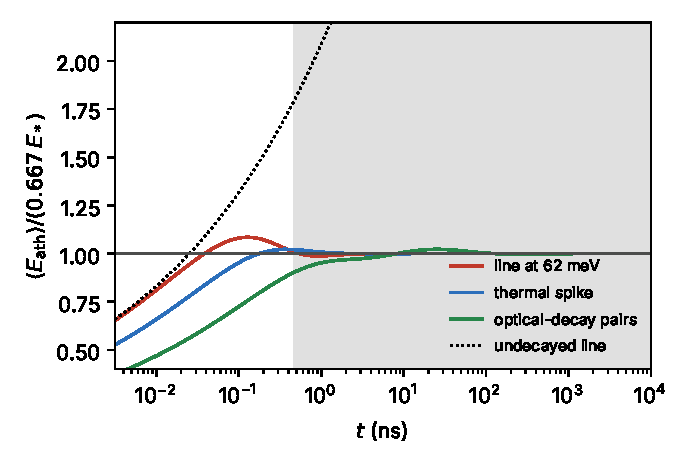
\includegraphics[width=0.75\linewidth]{figures/ch20/limit20_2a.pdf}
\captionof{figure}{Energy-weighted mean phonon energy in silicon divided by the scaling law $0.667\,E_*(t)$ of \cref{eq:20.2-Estar,eq:20.2-scaling}, against time, for three hard births (models): a line at the band top, \SI{62}{meV} (red); a spectrum growing as $E_{\mathrm{ath}}^3$ up to \SI{62}{meV} (blue); and the pairs of longitudinal (\SI{42}{meV}) and transverse (\SI{22}{meV}) phonons from optical decay, Gaussians of \SI{10}{\percent} relative width (green). Solution of \cref{eq:20.2-frag} with $f_{\mathrm{LA}} = 0.093$, $A_{\mathrm{anh}} = \SI{7.41e-56}{s^4}$, the daughter distribution $P_{\mathrm{d}}(y) = 60\,y^3(1 - y)^2$ and no surfaces, on a logarithmic grid of step 0.01 from 0.01 to \SI{18}{THz}, by the exact matrix exponential. Dotted: the leading correction at early times, the undecayed line, $(f_{\mathrm{LA}}A_{\mathrm{anh}}f_{\mathrm{top}}^5t)^{1/5}/0.667$. Gray: all three within \SI{10}{\percent}, $t \ge \SI{0.46}{ns}$.}\label{fig:20-limit-scaling}
\par}
\smallskip
Before the hardest phonons have decayed a few times the mean still depends on the birth spectrum; and where the continuum rates fail, above a few THz in silicon (\cref{lim:20.2b}), the time scale itself is an estimate.
\end{limitbox}

\subsection{Memory of the birth spectrum}\label{sec:20.2-memory}

How long does the birth spectrum leave a trace? We measure the trace by the total-variation distance between the normalized energy spectra that two births reach at time $t$, which is half the integral of their absolute difference. It bounds the difference of the energy that the two deliver into any part of the spectrum. Let $\Delta_{\mathrm{h}}(t)$ be its largest value over pairs of births above an energy $E_{\mathrm{mem}}$. By the scaling form $\Delta_{\mathrm{h}}$ depends on time only through $E_*(t)/E_{\mathrm{mem}}$, and the solutions of \cref{eq:20.2-frag} give the threshold: any two births above $E_{\mathrm{mem}}$ agree to $10^{-3}$ once $E_*(t)$ has fallen to between 0.51 and $0.53\,E_{\mathrm{mem}}$. A birth is forgotten when the scale has fallen to about half its energy, and since $E_* \propto t^{-1/5}$ the time this takes grows as the inverse fifth power of the birth energy. \Cref{fig:20-spectrum} shows the consequences for silicon.

\begin{figure}[tbp]
  \centering
  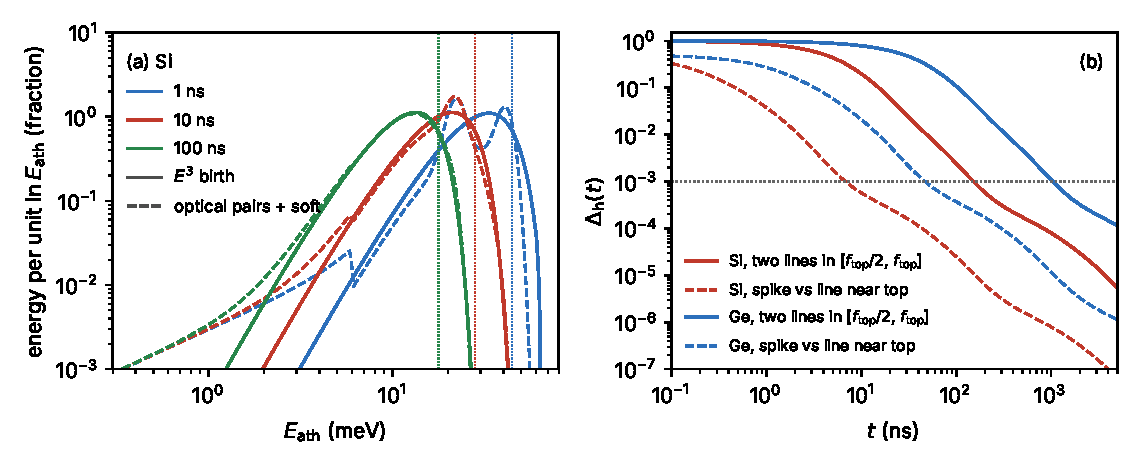
\includegraphics[width=\linewidth]{figures/ch20/fig20_2.pdf}
  \caption{Down-conversion of prompt phonons, from \cref{eq:20.2-frag} in the isotropic continuum with the mean decay rate $f_{\mathrm{LA}}A_{\mathrm{anh}}(E_{\mathrm{ath}}/h)^5$ for every phonon, the daughter distribution $P_{\mathrm{d}}(y) = 60\,y^3(1 - y)^2$ and no surfaces. (a) Energy spectrum of a silicon event, per unit $\ln E_{\mathrm{ath}}$ and normalized to the prompt energy, at 1, 10 and \SI{100}{ns} (colors), for two births (models). Solid: a spectrum growing as $E_{\mathrm{ath}}^3$ up to the band top, \SI{62}{meV}, standing for a locally thermalized nuclear recoil. Dashed: the longitudinal (\SI{42}{meV}) and transverse (\SI{22}{meV}) phonons of optical decay, Gaussians of \SI{10}{\percent} relative width with the energy shares 42:22 of the two phonons of an optical decay, plus the soft fraction $f_{\mathrm{s}} = \SI{1.7}{\percent}$ spread uniformly in energy over 0.2 to \SI{6}{meV}, standing for an electron recoil. Dotted verticals: $E_*(t)$. $A_{\mathrm{anh}} = \SI{7.41e-56}{s^4}$, $f_{\mathrm{LA}} = 0.093$. (b) Memory of the hard part, $\Delta_{\mathrm{h}}(t)$, for silicon (red) and germanium (blue; $A_{\mathrm{anh}} = \SI{1.61e-55}{s^4}$, $f_{\mathrm{LA}} = 0.098$, band top \SI{8.64}{THz}). Solid: the largest total-variation distance between two line births in the upper factor two of the band, $[f_{\mathrm{top}}/2, f_{\mathrm{top}}]$ (six lines). Dashed: one pair concentrated near the top, the $E_{\mathrm{ath}}^3$ spectrum against a Gaussian line at $0.95\,f_{\mathrm{top}}$ of width $0.05\,f_{\mathrm{top}}$. Dotted: $10^{-3}$, crossed by the dashed curves at \SI{6.8}{ns} (Si) and \SI{47}{ns} (Ge), and by the solid curves at \SI{0.15}{\micro s} (Si) and \SI{1.0}{\micro s} (Ge).}
  \label{fig:20-spectrum}
\end{figure}

The answer depends on how low the hard births reach. Take two births concentrated at the top of the band, the cubic spectrum and a line at \SI{95}{\percent} of the band top. They agree to $10^{-3}$ after \SI{6.8}{ns} in silicon and \SI{47}{ns} in germanium with its slowest decay constant (\cref{fig:20-spectrum}(b)), and the fastest germanium constant shortens the latter tenfold. Births spread over the upper factor two of the band take longer, \SI{0.15}{\micro s} in silicon and \SI{1.0}{\micro s} in germanium. The transverse phonons of optical decay, at \SI{22}{meV}, are forgotten only when $E_*$ has fallen to about \SI{11}{meV}, near \SI{1}{\micro s} in silicon. The two model births of \cref{fig:20-spectrum}(a) differ by a total-variation distance of 0.13 at \SI{10}{ns}, 0.026 at \SI{100}{ns}, 0.015 at \SI{300}{ns} and 0.012 at \SI{1}{\micro s}. At \SI{1}{\micro s} their parts above \SI{6}{meV} agree to $6\times10^{-4}$. What remains is the soft fraction: the electron recoil was born with \SI{1.7}{\percent} of its energy below \SI{6}{meV} and the cubic spectrum with \SI{0.01}{\percent}, and the decay of the hard parts has only begun to fill that region. All of these times rest on the continuum rates, which in silicon are applied at 5 to \SI{15}{THz}, above their range (\cref{lim:20.2b}), so they are estimates.

Polarization is forgotten much sooner. Along the scaling trajectory, the number of times a phonon has scattered off isotopes by the time $t$ is
\begin{equation}
  N_{\mathrm{mix}}(t) = \int_0^t\dd t'\,B_{\mathrm{iso}}\bigl[E_*(t')/h\bigr]^4 = 5B_{\mathrm{iso}}\,(f_{\mathrm{LA}}A_{\mathrm{anh}})^{-4/5}\,t^{1/5} ,
  \label{eq:20.2-Nmix}
\end{equation}
which is 164 at \SI{1}{ns} in silicon and 650 at \SI{1}{\micro s}; in germanium, with fifteen times the isotope constant, it is \num{1300} and \num{5100}. Each scattering redraws the branch from the equilibrium shares, so the fraction of phonons that still carry their birth branch is of order $\ee^{-N_{\mathrm{mix}}}$.

The phonons also spread out. Take the diffusion constant $v_{\mathrm{ph}}^2/3\varGamma_{\mathrm{iso}}$ of a gas with mean free time $1/\varGamma_{\mathrm{iso}}$ and rms group speed $v_{\mathrm{ph}}$, evaluated at $E_*(t)$. The mean squared distance from the event is then $6\int\dd t'\,v_{\mathrm{ph}}^2/3\varGamma_{\mathrm{iso}} = \frac{10}{9}v_{\mathrm{ph}}^2(f_{\mathrm{LA}}A_{\mathrm{anh}})^{4/5}t^{9/5}/B_{\mathrm{iso}}$. In silicon, with $v_{\mathrm{ph}} = \SI{5.85}{km/s}$, the rms distance is \SI{8.6}{\micro m} at \SI{10}{ns}, \SI{68}{\micro m} at \SI{100}{ns} and \SI{0.54}{mm} at \SI{1}{\micro s}. In germanium, with $v_{\mathrm{ph}} = \SI{3.52}{km/s}$, it is \SI{1.8}{\micro m}, \SI{15}{\micro m} and \SI{0.12}{mm}. This is the quasi-diffuse transport of athermal phonons~\cite[Sect.~2.2.2]{kelsey2023g4cmp}: the phonons random-walk while their mean free path grows with each decay, until it reaches the size of the crystal and they move ballistically. A phonon of \SI{45}{meV}, the binding energy of a phosphorus donor, belongs to a population that decays within \SI{0.95}{ns}, by which time it has spread over \SI{1.0}{\micro m}. An event closer to a sensor than the rms distance delivers part of its energy before its spectrum has settled, and there the birth is not forgotten. For a silicon detector \SI{4}{mm} thick with sensors on one face, such as that of Ren et al.~\cite{ren2021design}, that shell is \SI{0.21}{\percent} of the volume at \SI{10}{ns}, \SI{1.7}{\percent} at \SI{100}{ns} and \SI{13.5}{\percent} at \SI{1}{\micro s}. The memory times above decide how much of the volume counts as bulk.

Sapphire does not fit this picture. Its isotope constant is a hundred times smaller than that of silicon, $B_{\mathrm{iso}} = \SI{2.5e-44}{s^3}$ calculated and \SI{4e-44}{s^3} measured, while its decay constant lies between \num{1.88e-55} and \SI{1.27e-54}{s^4}. Hernandez et al.\ trace that spread to the anisotropy and to converting a published rate with the fifth power of a sound speed~\cite[Tables~3, 4]{hernandez2025modeling}. Compared to silicon, however, the hierarchy is reversed: mixing outpaces decay only below $B_{\mathrm{iso}}/A_{\mathrm{anh}} = 0.02$ to \SI{0.21}{THz}. Over the whole primary band a longitudinal phonon decays before it scatters, and the branches are not held at their equilibrium shares. A transverse phonon, which the isotropic continuum does not let decay, scatters $B_{\mathrm{iso}}(E_{\mathrm{ath}}/h)^4\times\SI{1}{\micro s} = 0.025$, 0.4 and 16 times in a microsecond at 1, 2 and \SI{5}{THz}. As a result, transverse phonons born below a few THz in sapphire keep their energy and their polarization for microseconds. The single rate $f_{\mathrm{LA}}\varGamma_{\mathrm{anh}}$ of \cref{eq:20.2-frag} does not exist, and the scaling argument fails at its first step. The fate of these phonons needs the decay rates of transverse phonons in an anisotropic crystal, which the isotropic continuum sets to zero.

\subsection{Transfer-kernel bound on observable differences}\label{sec:20.2-bound}

The memory of the spectrum matters through what a readout measures. Take an observable that is linear in the energies delivered to the sensors, with weights between zero and one: the fraction of the energy absorbed by one of two sensors, the fraction that arrives before a given time, or the collection efficiency of a population. Since the transport is linear, a birth spectrum $\hat\rho_0(E)$ normalized to unit energy gives $O = \int\dd E\,R_O(E)\,\hat\rho_0(E)$. Here $R_O(E)$, with $0 \le R_O \le 1$, is the value of the observable for unit energy born at $E$ at the event position, and \cref{sec:20.5} builds it from the collection kernels of a detector. Let $\Delta\hat\rho_0 = \hat\rho_0^{\mathrm{NR}} - \hat\rho_0^{\mathrm{ER}}$ be the difference of the birth spectra of the two recoils. Suppose that no sensor absorbs anything before a time $t_{\mathrm{mem}}$, and that births above $E_{\mathrm{mem}}$ have been forgotten by then, to the distance $\Delta_{\mathrm{h}}(t_{\mathrm{mem}})$ in energy, branch and position.
\begin{keyresult}[Transfer-kernel bound]
\begin{equation}
  |O^{\mathrm{NR}} - O^{\mathrm{ER}}| \le \int_0^{E_{\mathrm{mem}}}\dd E\,|\Delta\hat\rho_0(E)| + \Delta_{\mathrm{h}}(t_{\mathrm{mem}}) .
  \label{eq:20.2-bound}
\end{equation}
When $\Delta\hat\rho_0$ has one sign below $E_{\mathrm{mem}}$, the integral is $\Delta_{\mathrm{soft}} = |\int_0^{E_{\mathrm{mem}}}\Delta\hat\rho_0\,\dd E|$, the difference of the energy fractions born below $E_{\mathrm{mem}}$.
\end{keyresult}
\noindent The response to a birth above $E_{\mathrm{mem}}$ is the response to the state it has reached at $t_{\mathrm{mem}}$, and a weight between zero and one integrated against the difference of two normalized distributions is bounded by their total-variation distance. Two births $E_1$, $E_2$ above $E_{\mathrm{mem}}$ therefore have $|R_O(E_1) - R_O(E_2)| \le \Delta_{\mathrm{h}}$. Both birth spectra have unit energy, so $\int\Delta\hat\rho_0\,\dd E = 0$ and $O^{\mathrm{NR}} - O^{\mathrm{ER}} = \int(R_O - R_0)\,\Delta\hat\rho_0\,\dd E$ for any constant $R_0$. Choose $R_0$ midway between the largest and the smallest response above $E_{\mathrm{mem}}$. Then $|R_O - R_0| \le \Delta_{\mathrm{h}}/2$ above $E_{\mathrm{mem}}$, where $\int|\Delta\hat\rho_0| \le 2$, and $|R_O - R_0| \le 1$ below, which gives the two terms of \cref{eq:20.2-bound}. An observable that is a ratio of delivered energies, such as the share of one of two sensors, is linear to first order in the difference, and the range of its linearized weight replaces the factor one.

\Cref{eq:20.2-bound} names the one number that the created-phonon spectra of the two recoils must supply, the distance between their parts below $E_{\mathrm{mem}}$. The single-sign condition matters. Two births with the same energy below $E_{\mathrm{mem}}$ but different soft shapes, one just above the gap of a sensor film and one just below it, have $\Delta_{\mathrm{soft}} = 0$ and yet give different responses; the bound then needs the full $L^1$ distance. The branch content of a nuclear recoil above $E_{\mathrm{mem}}$ does not enter at all.

For the primary phonons the bound limits the spectral part of the collection offset of \cref{sec:19.5}. With the collection efficiency as the observable, $|\epsilon^{\mathrm{NR}}_{\mathrm{prim}} - \epsilon^{\mathrm{ER}}_{\mathrm{prim}}| \le \int_0^{E_{\mathrm{mem}}}|\Delta\hat\rho_0| + \Delta_{\mathrm{h}}$. If $E_{\mathrm{mem}}$ lies above the soft band and below every hard birth, and only the electron recoil carries a soft fraction, the integral is $f_{\mathrm{s}} = \SI{1.7}{\percent}$. The condition on $E_{\mathrm{mem}}$ is the weak point. For the model births of \cref{fig:20-spectrum}(a) at \SI{1}{\micro s}, the lowest energy above which births agree to $10^{-3}$, $E_{\mathrm{mem}} = \SI{21.6}{meV}$, cuts through the transverse daughters of optical decay, and the bound is 0.15, against an actual largest difference of 0.012. At \SI{3}{\micro s}, with $E_{\mathrm{mem}} = \SI{17.7}{meV}$, the bound has fallen to 0.026 against 0.009, but the near-face shell of a \SI{4}{mm} crystal is by then \SI{36}{\percent} of the volume. Within the bulk the spectral difference between the two recoils is set by the soft fraction and by how low the hard births reach; near an instrumented face this argument does not bound it.
